\documentclass[11pt]{report}
\usepackage{epsfig}
\usepackage{times}

\textwidth 159mm		% 16.2cm
\textheight 233mm		% 23.5cm
\hoffset 0cm
\voffset 0cm
\topmargin 0mm			% -1.5cm
\oddsidemargin 0mm
\evensidemargin 0mm

\title {\bf {\tt RenderPark} source code structure}
\date{November, 5 1999}
\author{Philippe Bekaert, Frank.Suykens \\
 Computer Graphics Research Group \\
 Departement of Computer Science \\
 K. U. Leuven, Leuven (Belgium) \\
 $\{$Philippe.Bekaert$|$Frank.Suykens$\}$@cs.kuleuven.ac.be}

\begin{document}
\maketitle

\chapter*{Introduction}

This document describes how the {\tt RenderPark} source code is structured.
It is meant as a starting point for people who wish to use
{\tt RenderPark} as a reference for their own implementations, or
who consider to implement
new (or old) rendering algorithms, using the large collection of 
``tools'' that are offered in {\tt RenderPark}. {\tt RenderPark} contains 
a large number of
recently and less recently proposed rendering algorithms. The
source code structure reflects that these rendering
algorithms are all built on top of a number of basic building blocks
that are common for many algorithms. An example of such a basic building block is
for instance the tracing of a ray in order to determine to
nearest intersection point along the ray with the surfaces of the scene.

Why is collaborating in a project like {\tt RenderPark} interesting?
\begin{itemize}
\item Sharing work is saving work: you don't have to do everything yourself
  as a lot things you need are already there, it is good for the quality of the
  implementations, allows to test each others work, it is an impulse to
  provide documentation (so others can use your work), leads
  to more careful design, a more efficient implementation of a common
  subtask is advantageous for all algorithms that are built
  on top of this subtask (e\@.g\@. ray-tracing acceleration schemes), \ldots;
\item It makes a fair comparison of rendering algorithms possible since
  all algorithms are built upon a common ``tool box'' and use the same 
  conventions \ldots
\item It makes interesting demonstrations;
\item {\tt RenderPark} is a prototype rendering engine, that should be 
  easy to tune for a particular application, and it can be a
  reference implementation for your rendering algorithms;
\item It's good publicity for your work and will be better publicity as more
  people use it;
\item \ldots
\end{itemize}
{\tt RenderPark} is made by global illumination researchers and is also mainly
targeted, but not restricted, to researchers in this exciting field.

This document contains two parts: first a part describing what can be
found in which source file (\S\ref{codestructure}), next a part describing
the main data structures (\S\ref{datastructures}). Section
\ref{radiance-methods} and \ref{raytracing-methods} present the actual 
implementation of rendering algorithms.

\chapter{Source code structure}
\label{codestructure}

\section{Main directory}

See figure \ref{fig1}. The main directory basically contains:
\begin{itemize}
\item the main program ({\tt main.c});
\item routines for reading {\tt MGF} and {\tt VRML'97} scenes 
  ({\tt main, readmgf, readvrml, PhBRML}), building
  a scene data structure and auxiliary structures (see \S\ref{datastructures}),
  saving an image in {\tt PPM} or {\tt TIFF} format, saving the ``illuminated''
  scene model after radiosity computations in {\tt VRML'97} format ({\tt writevrml}) 
  \ldots
\item everything of the graphical user interface that does not concern specific
  rendering algorithms ({\tt ui\_*}, X/Motif
  simplified with a small user interface toolkit in {\tt uit});
\item drivers for graphics hardware (OpenGL, IrisGL and starbase), manipulation
  of the virtual camera using the mouse, object selection (to update material 
  properties e\@.\@g.), \ldots ({\tt render,
  rendercommon, canvas, camera, \ldots}). Rendering algorithms that
  use graphics hardware for visualisation of the result shall fill in the
  colour to be used for each patch or vertex in the patch and vertex
  data structures that are offered ({\tt vertex\_type.h, patch\_type.h});
\item monitor calibration (to set monitor white point, gamma correction,
  and brightness adjustment) and tone mapping ({\tt color.c, eye.c});
\item command line option processing ({\tt options.*}), batch and offscreen
  rendering ({\tt batch}), Inter Process Communication control ({\tt ipc});
\item a ``tool box'' for rendering algorithms:
  \begin{itemize}
  \item ray-object intersection routines ({\tt geometry, grid, patch,
      shaftculling, shadowcaching});
  \item numerical integration on the square, triangle, 3D cube ({\tt cubature});
  \item ID-rendering, determination of directly received visual potential
    ({\tt render, potential}),
  \item uniform and $\cos\theta$ sampling of spherical triangles
    ({\tt spherical}), or patches ({\tt patch})
  \item KD-trees, transforms, line-plane and line-line intersection computation, \ldots;
  \item \ldots
  \end{itemize}
\item hooks for rendering algorithms: we make a distinction between 
  pixel-based rendering algorithms (such as stochastic ray tracing, 
  {\tt raytracing}) and world-space algorithms such as radiosity 
  ({\tt radiance}).
\end{itemize}

\begin{figure}
\begin{small}
\begin{verbatim}
0README              bsdf_methods.h       lightlist.C          shadowcaching.h
ARCHIVE              btdf.c               lightlist.H          shaftculling.c
BREP                 btdf.h               lightmetering.c      shaftculling.h
Boolean.h            btdf_methods.h       lightmetering.h      shooting.rw
ChangeLog            bzero.c              main.c               spectrum.h
Config.Alpha         camera.c             material.c           spectrum_type.h
Config.FreeBSD       camera.h             material.h           spherical.c
Config.HP            canvas.c             materiallist.c       spherical.h
Config.Linux         canvas.h             materiallist.h       splitbsdf.c
Config.SGI           cie.c                monitor.c            splitbsdf.h
Config.Solaris       cie.h                monitor.h            starbase.c
Config.common        cluster.c            motif.h              statistics.h
Config.site          cluster.h            mymath.h             stratification.C
Config.site.default  color.c              namedvertex.c        stratification.H
DEST                 color.h              namedvertex.h        sub.sh
DOC                  color.h.antiek       opengl.c             surface.c
Float.h              compound.c           options.c            surface.h
GALERKIN             compound.h           options.h            topology.c
GDT                  cubature.c           packedcolor.c        topology.h
GENETIC              cubature.h           packedcolor.h        transform.c
HURA                 defaults.h           patch.c              transform.h
IMAGE                deps                 patch.h              ui.h
MCRAD                edf.c                patch_flags.h        ui_camera.c
MCRAD.2              edf.h                patch_type.h         ui_canvas.c
MCRAD.stable         edf_methods.h        getPatchList.c          ui_config.c
MGF                  error.c              getPatchList.h          ui_debug.c
MGF-2.0a             error.h              patchlist_geom.h     ui_file.c
Makefile             eye.c                phong.c              ui_help.c
NON_PUBLIC           eye.h                phong.h              ui_main.c
PARTICLE             fileopts.h           polygon.h            ui_material.c
PHOTONMAP            fix.c                pools-1.4            ui_material.h
PNM                  fix.h                potential.c          ui_phong.c
POOLS                geometry.c               potential.h          ui_phong.h
PhBRML.C             geometry.h               radiance.c           ui_radiance.c
PhBRML.H             geom_methods.h       radiance.h           ui_raytracing.c
QMC                  geom_type.h          ray.h                ui_render.c
RAYTRACING           geometry3d.c         raycasting.h         uit.c
RenderPark           geometry3d.h         raytracing.c         uit.h
SCENES               geomlist.c           raytracing.h         vector.c
SE                   geomlist.h           readmgf.c            vector.h
SGL                  gl.c                 readmgf.h            vectorlist.c
TODO                 grid.c               readvrml.C           vectorlist.h
TOOLS                grid.h               readvrml.H           vectoroctree.h
ad2c.script          gridP.h              render.h             vectortype.h
appdata.h            hemirenderer.C       rendercommon.c       vertex.c
batch.c              hemirenderer.H       renderhook.c         vertex.h
batch.h              hitlist.c            renderhook.h         vertex_type.h
bidir-lab.fig        hitlist.h            renderhook_priv.h    vertexlist.c
bidir-lab.fig.bak    hitlist_type.h       rgb.h                vertexlist.h
getBoundingBox.c             ipc.c                rtdummy.C            writevrml.c
getBoundingBox.h             ipc.h                rtdummy.h            writevrml.h
brdf.c               jacobian.c           scene.c              xxdf.c
brdf.h               jacobian.h           scene.h              xxdf.h
brdf_methods.h       kdtree.C             select.c
bsdf.c               kdtree.H             select.h
bsdf.h               lib                  shadowcaching.c
\end{verbatim}
\end{small}
\caption{Files in the {\tt RenderPark} main directory}
\label{fig1}
\end{figure}

%\end{verbatim}
%\end{figure}
%
%\begin{figure}
%\begin{verbatim}

\section{subdirectories}

\begin{itemize}
\item {\tt DOC/}: documentation;
\item {\tt TOOLS/}: sub-directory for small test programs and tools for 
  e\@.g\@. comparing images. Does not contain code that is needed to
  build the {\tt RenderPark} executable
\item Auxiliary libraries:
  \begin{itemize}
\item {\tt GDT/}: generic data types (in C, to be superceeded by C++ sometimes 
  in the future);
\item {\tt POOLS/}: memory management;
\item {\tt MGF/}: MGF parser library;
\item {\tt SGL/}: Simple Graphics Library (for clustering in Galerkin radiosity methods e\@.g\@., also useful for other purposes);
\item {\tt BREP/}: Boundary REPresentatie library;
\item {\tt QMC/}: low-discrepancy (quasi-Monte Carlo) number generators;
\item {\tt SE/}: contains ply file format library + simplify program needed
	for mesh decimation in density esitmation.
\item {\tt IMAGE}: Image output in PPM or TIFF format.
\end{itemize}
\item Actual implementation of rendering algorithms:
  \begin{itemize}
  \item {\tt GALERKIN/}: Galerkin radiosity;
  \item {\tt MCRAD/}: Monte Carlo radiosity: Hierarchical WDRS, Random
	Walk Radiosity and Stochastic Ray Radiosity;
  \item {\tt RAYTRACING/}: ray-casting, classical and stochastic raytracing;
  \item {\tt DEST/}: Density Estimation (contributed by Olivi\'e Ceulemans,
	UCL/KUL Belgium);
  \item {\tt HURA/}: The Ultimate Rendering Algorithm (Het Ultieme Rendering Algoritme): 
    for the time being just a template that you can copy to add your own
    rendering algorithms to {\tt RenderPark}.
  \end{itemize}
  The rule is that subdirectories can use data structures and global variables
  from their parent directory, but not vice versa, except
  for the auxiliary libraries such as {\tt GDT} and {\tt POOLS}.
\end{itemize}

\section{Adding a new rendering algorithm}

\begin{itemize}
\item First decide what class your rendering algorithm belongs to:
  world-space or pixel-based. This determines what routines (``methods'') 
  you have to implement in order to hook up your algorithm in the 
  {\tt RenderPark} program and how it will fit in the user interface. 
  Suppose you want to add a world-space algorithm (adding
  a pixel-based algorithm is similar);
\item make a separate sub-directory for your algorithm and copy
  the (template) files in the {\tt HURA} sub-directory. Change the name 'hura'
  to something of your own;
\item add a pointer to your rendering algorithm handle to the table of
  supported algorithms in {\tt radiance.c}. If you want to add a
  pixel-driven algorithm, update {\tt raytracing.c};
\item change the Makefile in order to compile and link you code as well
  when you do 'make' in the main directory;
\item of course, implement the methods defined in {\tt radiance.h}
  or {\tt raytracing.h}.
\end{itemize}

\chapter{Data structures}
\label{datastructures}

\section{The scene data structure}

Scenes are represented using the following data structures and global
variables (declared in {\tt scene.h}):
\begin{itemize}
\item   A linear list of material descriptions:
        \newline
        {\tt MATERIALLIST *GLOBAL_scene_materials}
        \newline
        The type {\tt MATERIALLIST} represents a linear list of material
        descriptions {\tt Material} and is declared in
        {\tt materiallist.h}. The type {\tt Material} is declared in
        {\tt material.h}. See also below, \S\ref{material}.
\item   A linear list of geometries:
        \newline
        {\tt GeometryListNode *GLOBAL_scene_world}
        \newline
        The type {\tt GeometryListNode} ({\tt geomlist.h}) is a
        linear list of {\tt Geometry} structures ({\tt geometry\_type.h}).
        A {\tt Geometry} structure represents all information about a
        geometry (object), see \S\ref{geometry}.
\item   A couple of data structures derived from the above when
  reading in a new scene:
  \begin{itemize}
  \item {\tt PatchSet *GLOBAL_scene_patches}: linear list of all patches making up together
    the whole scene;
  \item {\tt Geometry *GLOBAL_scene_clusteredWorldGeom}: hierarchical scene representation with
    an automatically generated and most often better GLOBAL_stochasticRaytracing_hierarchy of bounding
    boxes;
  \item{\tt VoxelGrid *GLOBAL_scene_worldVoxelGrid}: the scene packed into a voxel grid for
    raytracing acceleration ({\tt grid}).
  \end{itemize}
\end{itemize}
Lists and other data structures such as binary trees, octrees, \ldots
are derived (using macros, see e\@.g\@. {\tt getPatchList.h})
from a generic implementation in the {\tt GDT} (Generic Data Types) library.

\section{The {\tt Geometry} type}
\label{geometry}

There are basically two types of geometries in the program:
\begin{itemize}
\item   {\tt Compound} objects ({\tt compound.h}: an aggregate object:
  basically a list of constituting {\tt Geometry}etries, see \S\ref{compound};
\item   {\tt MeshSurface}s ({\tt surface.h}): a primitive objects: basically
  a list of {\tt Patch}es ({\tt patch.h}) that approximate the
  surface of some object, see \S\ref{surface};
\end{itemize}
{\tt Geometry} should be seen as a superclass of {\tt Compound} and {\tt MeshSurface}.
The implementation is in C and not C++ for historical reasons. We consider
reimplementing everything in C++, after redesigning the whole scene
representation data structure. This has quite low priority however
because the current implementation fulfills our needs well and has
proven to be pretty reliable.

The {\tt Geometry} structure ({\tt geometry\_type.h}) contains:
\begin{itemize}
\item   A pointer to object-specific data:
        \newline
        {\tt void *genericAttachedData}
        \newline
        For compound objects, it is a pointer to a {\tt Compound}
        struct ({\tt compound.h}), for a surface object, it is a pointer
        to a {\tt MeshSurface} struct ({\tt surface.h});
\item   A pointer to a {\tt Geometry\_METHODS} struct ({\tt geometry\_methods.h}).
  This structure contains pointers to a set of functions (methods) for 
  manipulating the object data. This ``methods'' have the same interface for
  all kind of objects, but, of course, the implementation is different for 
  different types of objects. For compound objects, the methods are
  implemented in {\tt compound.c}, for surfaces in {\tt surface.c}.
  Some examples of methods: ray-object intersection testing, requesting
  a list of constituting geometries (for a compound object), \ldots
\item   A bounding box (type {\tt BOUNDINGBOX}, see {\tt getBoundingBox.h}).
\item   A pointer to data for the geometry that are specific for a given
  rendering algorithm. When you need to associate specific data with a 
  geometry in your rendering algorithm, you allocate space for this data
  and fill in this pointer for each geometry in the scene when initialising
  your algorithm. When terminating, you need to dispose of the allocated
  storage and set the pointer to {\tt NULL} again. The pointer is initialised
  to {\tt NULL} when reading in a scene. (see also {\tt radiance.h} or
  the example in the {\tt HURA/} sub-directory).
\end{itemize}

\section{{\tt Compound}s}
\label{compound}

The object specific data for a compound object is nothing else than
a pointer to a linear list containing the constituting {\tt Geometry}etries.
These constituting geometries may be surfaces or again compound objects, so
you can build a hierarchical representation of your scene.

\section{{\tt MeshSurface}s}
\label{surface}

Besides an identification number, useful for debugging, a {\tt MeshSurface}
struct contains:
\begin{itemize}
\item   a {\tt Material *material} pointer to the material description
  of the object;
\item   a linear list {\tt Vector3DListNode *positions} of coordinates of patch
  vertices;
\item   a linear list {\tt Vector3DListNode *normals} of vertex normal vectors;
\item   a linear list {\tt VERTEXLIST *vertices} of vertex descriptions
  (see \S\ref{vertices});
\item   a linear list {\tt PatchSet *faces} of the patches that together
  make up the surface (see \S\ref{patches}).
\end{itemize}

\section{Vertices: the {\tt Vertex} type}
\label{vertices}

For each vertex of a patch, the following information is kept ({\tt vertex.h}):
\begin{itemize}
\item   a pointer {\tt Vector3D *point} to the vertex coordinates. Coordinates
  can be shared by several vertices. We store the coordinates only once
  for saving storage. It is also more efficient to compare a pointer to
  the coordinates than to compare the coordinates themselves if you want to
  know if two vertices have the same coordinates;
\item   a pointer {\tt Vector3D *normal} to the vertex normal if specified in the
  input file, or {\tt NULL} if no vertex normal was specified;
\item   a linear list {\tt PatchSet *patches} of patches sharing the vertex.
  Useful for computing a vertex color as the average color of the patches
  sharing the vertex for smooth shading e\@.g\@.;
\item   a color ({\tt RGB} type) to render the vertex when using Gouraud
  interpolation. This color needs to be computed and filled in the {\tt Vertex}
  structures by your rendering algorithm if you want to use the existing
  routines for smooth shaded rendering with graphics hardware;
\item   a pointer to rendering algorithm specific data attached to the
  vertex. This pointer is initialised to {\tt NULL} when reading a scene
  and needs to be set to {\tt NULL} again after you dispose of the data
  you attached to the vertex when your rendering algorithm is terminated.
  It is used in the same way as rendering algorithm specific data for 
  {\tt Geometry}etries.
\end{itemize}

\section{Faces: the {\tt Patch} type}
\label{patches}

This very crucial data type, declared in {\tt patch\_type.h}, contains
besides some less important things:
\begin{itemize}
\item   an ID-number for debugging and ID-rendering;
\item   an array {\tt Vertex *vertex[MAXIMUM_VERTICES_PER_PATCH]}
        of {\tt MAXIMUM_VERTICES_PER_PATCH} (=4) pointers to the vertices of
        the patch (last pointer is a {\tt NULL} pointer for triangles);
\item   the number of vertices (3 or 4);
\item   a back-pointer {\tt MeshSurface *surface} to the surface to which the
  patch belongs. Useful to find the material characteristics e\@.g\@.;
\item   a bounding box: this is a {\tt NULL} pointer until a bounding box
  is needed the first time;
\item   patch plane normal and plane constant, midpoint, index of dominant
  normal component, jacobian of parameter transform, \ldots
\item   a color {\tt RGB color}: to be filled in by your rendering algorithm
  in order to use graphics hardware for rendering your results;
\item   a pointer to rendering algorithm specific data for the patch, used
  in the same way as vertex or geometry specific data {\tt radiance.h};
\item   \ldots
\end{itemize}

\section{Materials: the {\tt Material} type}
\label{material}

Besides a name for the material and an indication whether or not to consider
surfaces of the given material as two-sided or one-sided surface, the
{\tt Material} type contains pointers to
two functions that model the optical characteristics of the surface:
\begin{itemize}
\item {\bf Emittance Distribution Function}: only defined for light sources.
  Determines how intense light is emitted by a light source as a function
  of direction;
\item {\bf Bidirectional Scattering Distribution Function}: describes
  how light is scattered (reflected or broken) at a given surface.
\end{itemize}
The corresponding data types {\tt EDF} ({\tt edf.h}) and
{\tt BSDF} ({\tt bsdf.h}) are base classes
in the same way as {\tt Geometry} is a base class for {\tt Compound} and
{\tt MeshSurface}. These base class structs basically contain a pointer to
instance data and to methods to operate on the data.

\subsection{Material data}

The EDF/BSDF representation depends on the input file format (MGF or VRML).

MGF supports only a diffuse EDF and Phong-like reflection and refraction.
The BSDF consists of separate data for reflection and
refraction ({\tt splitbsdf.[ch]}):
\begin{itemize}
\item {\em Bidirectional Reflectance Distribution Function}: describes how
  intense light coming from a first direction is being reflected into a 
  second direction. Only defined for reflective materials;
\item {\em Bidirectional Transmittance Distribution Function}: describes
  how intense incident light from a given first direction is being transmitted
  into a second direction (pointing into the other side of the material).
  Only defined for transparent materials;
\end{itemize}
Also {\tt BRDF} ({\tt brdf.h}) and {\tt BTDF} ({\tt btdf.h}) are base classes,
similar to {\tt BSDF} \ldots. The implementation of the Phong-like BR/TDF can be
found in {\tt phong.c}.

VRML'97 is being extended with a very flexible and general EDF and BSDF model,
extending the simple OpenGL-like material model that is available in the standard.
The representation of this material model is not a part of RenderPark, but is
kept in a separate library. The interface to this library can be found in
{\tt readvrml.C} and {\tt PhBRML.C}.

\subsection{Material methods}

Besides routines for creating, printing, duplicating and destroying material data,
the main EDF methods are:
\begin{itemize}
\item	{\em Evaluation} of the EDF for a given point in space and (outgoing) direction;
\item	{\em Sampling} of a outgoing direction at a given point. Besides the sampled 
	direction, also the probability density of generating the direction is
	returned.
\item	Computation of {\em emittance}: the integral of EDF times cosine w\@.r\@.t\@.
	the surface normal over the full hemisphere at a given point on a surface
	in the scene.
\end{itemize}
A distinction is made between diffuse, directional diffuse (glossy) and
specular emission.

The main BSDF methods are:
\begin{itemize}
\item	{\em Evaluation} of the BSDF at a given point of a surface of the scene and
	for given incoming and outgoing directions;
\item	{\em Sampling} of a outgoing direction for given incoming direction at a given
	point. Besides the sampled outgoing direction, also the probability
	density of generating the direction is required;
\item	Computation of the {\em albedo}: the integral over all outgoing directions of
	the BSDF for given incoming direction at a given point;
\item	Computation of the {\em refraction index} at a given point on a transparant surface.
\end{itemize}
In the former three routines, a restriction can be made to any combination of
\begin{itemize}
\item	{\em reflection} or {\em refraction};
\item	{\em diffuse} or {\em directional diffuse (glossy)} or {\em specular} 
	component.
\end{itemize}
A restriction to only emission, reflection or refraction in any of the 
three glossiness ranges is needed for multipass methods.
A radiosity algorithm will compute only diffuse illumination
components. A second globalPass raytracing method will add the glossy and
specular component. The ``glossy'' component can be computed and stored 
with radiosity-like algorithms but the border between glossy and specular
is furthermore arbitrary. (Finite-element methods for directional diffuse environments
have not yet been implemented in RenderPark.)

The implementation of these methods is in {\tt phong.c} for the modified Phong
model in MGF, and in the VRML library for VRML'97. The interface to the VRML material
library is in {\tt PhBRML.C}.

\chapter{GLOBAL_currentRadianceMethodHandle methods}
\label{radiance-methods}

This section describes the actual implementation in RenderPark of world-space based
rendering algorithms.

\section{The radiance methods interface}

All world-space based rendering algorithms provide an implementation of the 
interface defined in {\tt radiance.h}. The main elements of this interface
are:
\begin{itemize}
\item	name of the world-space based rendering algorithm and other data for
	user interface buttons and command line options;
\item	a routine that initialises global variables of the algorithm to 
	a default value. This routine is called once during initialisation of
	RenderPark, before loading scenes and before the user interface is created;
\item	a routine to parse and to print command line options for the algorithm;
\item	a routine that initialises the algorithm whenever a new scene is loaded
	or when the user selects the rendering algorithm for an already loaded scene:
	for instance, initialisation of radiosity data for each patch in the scene;
\item	a routine to perform one step of the computations, for instance one iteration
	of a radiosity algorithm;
\item	a routine to terminate the computations with the algorithm on the given scene.
	This routine frees all memory that was explicitely allocated in the 
	initialisation routine or during the computations;
\item	a routine returning the radiance emitted at a given point on a given patch
	and into a given direction (for multipass methods or ray-casting of the result
	for instance);
\item	optional 
	routines to allocate memory for algorithm-specific data to be associated
	with each patch in the scene, to printRegularHierarchy this data, and to free this memory.
	The allocation routine is called for every patch in the scene before the
	initialisation routine is called when loading a new scene, or selecting
	the algorithm for rendering an already loaded scene. These routines
	are not required: the same work could be done by the
	initialisation/termination routines, but they are sometimes convenient;
\item	routines for creating, destroying and displaying a control panel for the
	rendering algorithm, in order to let the user set options and parameters
	of the algorithm;
\item	a routine that shows a panel with statistics information about a run of
	the algorithm, for instance computation time, memory usage, \ldots;
\item	a optional routine to render the scene if the default hardware-based rendering
	routine is not sufficient. If this routine is not implemented, default
	hardware-based rendering ({\tt render.c, rendercommon.c}) is used. The
	default rendering routine expects that a display RGB colour is filled in
	for every patch and vertex in the scene. A radiosity method for instance
	will compute and fill in these colour values and use the default rendering
	routine for display of the result;
\item	a routine to recompute display RGB colours of vertices and patches after 
	for instance a change of the gamma correction parameter in the monitor
	calibration panel;
\item	a routine that allows the rendering algorithm to react on a change of
	material characteristics, currently unused;
\item	an optional routine to save the result of the computations in a VRML'97
	file. This routine is only needed if the default VRML'97 saving 
	routine ({\tt writevrml.c}) is not sufficient. In general, a rendering
	algorithm will need both its own display routine and VRML saving routine,
	or none of both.
\end{itemize}


\chapter{Raytracing methods}
\label{raytracing-methods}


\section{Adding a ray tracing method}

{\bf struct Raytracer}: (raytracing.h) Provide a number
of functions and data for a new raytracing method.


\begin{itemize}

\item{\bf Variables}
\begin{itemize}
\item {\bf char *shortName}: Short name for the raytracing method, for use 
	as argument of raytracing command line option.

\item {\bf int nameAbbrev}:  how short can the short name be abbreviated? */

\item {\bf char *fullName}:  Full name of the raytracing method.

\item {\bf char *buttonName}: Name for the button for activating the method 
	in the raytracing method menu.
\end{itemize}

\item{\bf Initialisation \& Termination}
\begin{itemize}
\item {\bf void (*lightnessDefaults)(void)}: Function for setting default values etc...
	Called only upon startup of RenderPark. So switching between methods
	does not revert to default settings.

\item {\bf void (*parseOptions)(int *argc, char **argv)}: Function for parsing
	method specific command line options.

\item {\bf void (*PrintOptions)(FILE *fp)}: Function for printing method 
	specific command line options

\item {\bf void (*Initialize)(void)}: Initializes the current scene for 
	raytracing computations.  Called when a new scene is loaded or
	when selecting a particular raytracing algorithm.

\item{\bf void (*trwfTerminate)(void)}: lightnessTerminate raytracing computations. Free up any
	memory that is still allocated for the method. Called when another
	raytracing method becomes active or upon exit.
\end{itemize}


\item{\bf Computing an image}
\begin{itemize}

\item {void (*Raytrace)(ImageOutputHandle *ip)}: Raytrace the current 
	scene as seen with the current camera. If 'ip' is not a NULL
	pointer, write the raytraced image using the image output
	handle pointerd to by 'ip'.

\item {void (*InterruptRayTracing)(void)}: Interrupts raytracing as soon as
	possible. (Normally sets an 'interrupt' flag)
\end{itemize}

\item{\bf Image control}
\begin{itemize}

\item {\bf int (*rayCasterRedisplay)(void)}: Redisplays last raytraced image.
	Returns FALSE if there is no previous raytraced image and TRUE
	there is.


\item {\bf int (*rayCasterSaveImage)(ImageOutputHandle *ip)}: Saves last raytraced
	image in the file describe dby the image output handle.
\end{itemize}

\item{\bf User interface}
\begin{itemize}

\item {\bf void (*CreateControlPanel)(void *parent\_widget)}: Function for 
	creating user interface panel for interactively setting method
	specific parameters parent widget is passed as a void *. The
	type is however 'Widget', but we don't want to include the Xt
	header files in interface-independent files.

\item {\bf void (*ShowControlPanel)(void)}: Show user interface control panel.
	Called when 'Control' button in raytracing menu is selected.
\item {\bf void (*HideControlPanel)(void)}: Hide user interface control panel
\end{itemize}
\end{itemize}

To add a method provide a new 'Raytracer' structure and
all the needed functions and add the new method to 'raytracing.c'


\section{Utility classes/function for ray tracing}

\subsection{Screen iterator (screeniterate.C/H)}

Utility functions to iterate all pixels in the image.
A callback function must be provided that is called
for every pixel in the image.
The iterate functions show results on screen, but do not
store the image!

Current available functions:

\paragraph{void ScreenIterateSequential(SCREENITERATECALLBACK callback, void *data)}

Iterate pixels from top left to bottom right.

\paragraph{ScreenIterateProgressive(SCREENITERATECALLBACK callback, 
			      void *data)}

'Progressive' evaluation of pixels. 


\subsection{Class PathNode}

A path node is one vertex in a path. PathNode contains
all necessary information needed for evaluation of paths.
E.g. hit point, hit surface, normal, bsdf evaluation,
incoming direction, depth, pointer to next and previous node, \ldots

\subsection{Sampler Classes}

Sampler classes are used for building and extending paths.
The most important function in these classes is 'Sample'
which fills in a new path node, possibly depending on a
current and previous path node.

Function:
{\tt virtual bool Sample(PathNode *prevNode, PathNode *thisNode,
  PathNode *newNode, double x\_1, double x\_2); }


All 'sample' functions return a boolean value that indicates if
the new node is filled in. 'x\_1' and 'x\_2' are random numbers from
0.0 to 1.0.

Files: eyesampler.C/H


There are a number of different samplers available, all with
a different purpose


\subsubsection{Eye sampler}

sample a point on the eye surface. Currently a pinhole
camera model is used, so that this sampler fills in the pathnode
with the eye point.

Files: eyesampler.C/H

\subsubsection{Pixel sampler}

sample a random point on a pixel. Trace a ray through that point
and find the nearest intersection point. The new path node is filled
in with information from this intersection point.

Files: pixelsampler.C/H

\subsubsection{MeshSurface samplers}

MeshSurface samplers fill in the new path node with a point somewhere
in the scene that is usually generated by sampling a direction
and tracing a ray from the current path node in that direction.

Files: bsdfsampler.C/H, specularsampler.C/H

\subsubsection{Light sampler}

A light sampler samples a certain point on a light source. This
is used for next event estimation (Stoch. Raytracing) and
for generating starting point for light paths (Bidir. path tracing).

Files: lightsampler.C/H

\subsubsection{Light direction sampler}

The current path node should be on a light source. A direction
is chosen an a ray traced. A new path node is filled in with
the new hit point information.

Files: lightdirsampler.C/H


\subsection{Class ScreenBuffer}

Class for storing pixel radiance information. 
Method examples are 'add radiance/flux to a specified pixel', '
render the buffer to screen (converts radiance to rgb)', 'save buffer
as ppm or high dynamic range tiff', \ldots

Files: screenbuffer.C/H


\section{Example: Tracing of add path}

\begin{figure}[h]
  \begin{center} 
        \leavevmode 
          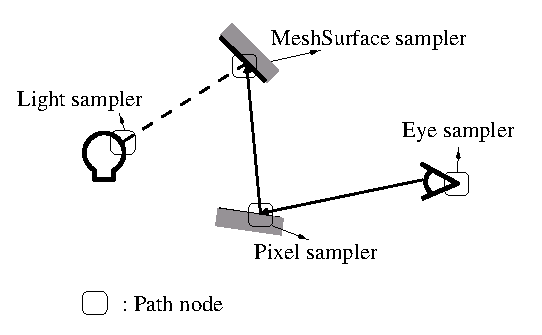
\epsfig{file=./rpkrt_fig.eps}
        \caption{Example of how a path is traced and which samplers
	are used to create/fill in the respective path nodes} 
        \label{f_rpkfig} 
  \end{center}
\end{figure}

\end{document}
